\documentclass[aps,prd,twocolumn,showpacs,superscriptaddress,nofootinbib]{revtex4-2}

\usepackage{amsmath,amssymb}
\usepackage{graphicx}
\usepackage{booktabs}
\usepackage{siunitx}
\usepackage{hyperref}

% Canonical counts from scripts/update_counts.py.
% Do NOT hardcode theorem/module counts inline — use macros.
% Auto-generated by update_counts.py — 2026-04-24T19:44:03.140400
% Do not edit manually. Run: uv run python scripts/update_counts.py
\newcommand{\totaltheorems}{3993}
\newcommand{\substantivetheorems}{3882}
\newcommand{\placeholdertheorems}{111}
\newcommand{\axiomcount}{1}
\newcommand{\sorrycount}{0}
\newcommand{\sorrypercent}{0.0}
\newcommand{\leanmodules}{167}
\newcommand{\leandefinitions}{3297}
\newcommand{\pythonmodules}{68}
\newcommand{\testfiles}{59}
\newcommand{\totaltests}{2836}
\newcommand{\figurecount}{111}
\newcommand{\notebookcount}{54}
\newcommand{\papercount}{19}
\newcommand{\aristotleproved}{322}
\newcommand{\aristotleruns}{44}
% --- Paper 18 / Phase 5t per-section counts (FermiHubbardDimer.lean) ---
\newcommand{\fhdTotal}{143}
\newcommand{\fhdWaveTwo}{13}
\newcommand{\fhdWaveThree}{6}
\newcommand{\fhdWaveFour}{22}
\newcommand{\fhdWaveFive}{22}
\newcommand{\fhdWaveSixABC}{38}
\newcommand{\fhdWaveSixExtra}{15}
\newcommand{\fhdWaveSeven}{19}
\newcommand{\fhdWaveEight}{8}


\begin{document}

\title{Dark Sector Connections from Emergent Gravity:\\
Machine-Verified Constraints from the SK-EFT Hawking Program}

\author{SK-EFT Hawking Research Program}

\date{\today}

\begin{abstract}
We present a unified assessment of how the effective field theory (EFT)
infrastructure developed in the SK-EFT Hawking research program—%
Schwinger--Keldysh dissipative EFT, tetrad condensation (ADW), vestigial
gravity phase structure, $\mathbb{Z}_{16}$ anomaly computation, and
fracton formalization—constrains dark matter (DM) and dark energy (DE).
Four connections are quantitative and machine-verified: (i)~$\mathbb{Z}_{16}$
anomaly cancellation forces a hidden sector of charge $+3 \bmod 16$, with
Wang's topological order (T-0) and three sterile Weyl fermions (S-0) as
the minimal solutions; (ii)~ADW tetrad-condensation equilibrium yields
$\rho_{\rm vac} \sim T^4 \sim (\mathrm{meV})^4$, reproducing the
observed cosmological-constant scale at the order-of-magnitude level
(the $\mathcal{O}(1)$ prefactor is deferred to Phase 6; a prior
``$20\%$'' agreement claim is withdrawn in this revision); (iii)~fracton dark
matter is compatible with $3{+}1$D gravity through the gapless p-wave
dipole superfluid phase, subject to a condensate condition $\mu \gtrsim
\SI{}{\mega\electronvolt}$ at big bang nucleosynthesis (BBN); and
(iv)~superfluid dark matter (SFDM) cluster mergers at the Berezhiani-Khoury
(BK) fiducial produce a supersonic sonic-boom feature observable at
$3{-}5\sigma$ by Euclid or Roman stacking of~$N \gtrsim 30$ radio-relic
mergers, with a velocity-threshold step function at~$M{=}1$ as an SFDM-unique
smoking gun. Every Phase 5x dark-matter candidate is Standard-Model gauge singlet
(derived from the fracton--Yang--Mills incompatibility theorem) and,
given deep-research $\sigma_{\rm DD}$ bounds for each candidate,
collectively below the current nuclear-recoil direct detection floor,
$\log_{10}\sigma_{\rm DD}(\SI{}{\centi\meter\squared}) \leq -50$.
The Klinkhamer--Volovik (KV) oscillating vacuum is in $2.9{-}4.4\sigma$
tension with DESI DR2 $(w_0, w_a)$; we retain the $\Lambda$-magnitude
prediction and withdraw the DE-dynamics claim. Structural claims split
into two Lean classes: \emph{derived} theorems whose proofs consume
physics assumptions (SM-singlet from fracton--YM, equation-of-state
distinctness from the rationals $w\!\in\!\{-1, 0, 1/3\}$, FG tree-level
CDM obstruction from traceless $T^{\mu\nu}$) and \emph{machine-checked
classifications} (MCC) — the candidate-viability matrix, the
collective-invisibility cap, the two-torsion-channel identification,
and the empirical-hook priority ordering — which encode the deep-
research classifications as a Lean lookup table and verify internal
consistency. (\emph{DarkSectorSynthesis.lean} and \emph{SFDMMergerForecast.lean}
together ship the Phase 5x synthesis; full per-module theorem counts
are machine-maintained in \texttt{docs/counts.tex} and
\S\ref{sec:formal-verification}.) The MCC class is not a physics
derivation; its purpose is to make the Phase 5x classification machine-
auditable and keep the paper's honesty table enforceable. See
\S\ref{sec:formal-verification} and Table~\ref{tab:honesty} for the
MCC--vs--Derived boundary.
\end{abstract}

\maketitle

%% ================================================================
\section{Introduction}
\label{sec:intro}

Analog-gravity research has produced an EFT toolkit for horizon physics
that is increasingly free of ad-hoc assumptions: Unruh--Visser acoustic
metrics~\cite{Unruh1981,Visser1998}, the Crossley--Glorioso--Liu
Schwinger-Keldysh framework for dissipative corrections~\cite{CGL2017a,CGL2017b},
and Volovik's tetrad-condensation viewpoint on vacuum
energy~\cite{Volovik2006,KV2008}. Meanwhile, machine-verified mathematics
has matured to the point where topological quantum field theory, bordism
invariants, and anomaly classification are within reach of interactive
theorem provers~\cite{Lean4,Mathlib}. Papers~1--16 of this series formalized
each of these components as Lean~4 theorems with zero \texttt{sorry}.

This paper asks which dark-sector (DM + DE) claims are derivable from the
verified program, and which are heuristic extrapolations that use it only
as a motivation. We find four derivable results and one heuristic one,
organized by the underlying theoretical structure:
\begin{itemize}
\item \emph{Anomaly cancellation.}~The $\mathbb{Z}_{16}$ global anomaly of
the Standard Model~\cite{Wan2019,Wang2020,Garcia-Etxebarria2019} forces a
hidden sector of charge~$+3 \bmod 16$—the remainder after three generations
contribute~$-3$. The hidden sector can be a topologically-ordered gapped
phase (T-0) or a minimal particle solution (S-0: three sterile Weyl
fermions).
\item \emph{Tetrad condensation and the cosmological constant.}~The ADW
gap equation~\cite{ADW2019,Diakonov2011}—a Volovik-style mean-field
equation for emergent gravity—has a critical point at $C_0 = \Lambda
e^{-1/4}$ with $V_{\rm eff}(C_0) = -\Lambda^4 / (4e)$. The residual
equilibrium value after thermal perturbation is~$\rho_{\rm vac} \sim T^4$.
\item \emph{Fracton dark matter.}~Our earlier formalization of
non-Abelian fracton obstructions~\cite{FractonNonAbelian2025} proves that fracton
topological phases cannot support Yang--Mills, so any fracton DM must be
SM gauge singlet. Recent work~\cite{Kapustin2022,Jensen2024,Glodkowski2024,%
Feistl2026} establishes that the p-wave dipole superfluid phase is
thermodynamically stable in $d{\geq}3$ at~$T{>}0$, resolving the
earlier finite-$T$ no-go~\cite{Krishna2024}.
\item \emph{Superfluid dark matter mergers.}~The BK~\cite{BK2015,BK2025}
fiducial sound speed $c_s = \SI{1525}{\kilo\meter/\second}$ at the
sub-cluster scale places all five canonical radio-relic cluster mergers
(Bullet, El Gordo, Pandora, A520, MACS J0025) in the supersonic regime.
A Rankine--Hugoniot analysis at the SFDM effective adiabatic index
$\gamma_{\rm eff}{=}2$ yields a condensate density jump~${\sim}49\%$.
Stacking~$N \gtrsim 30$ such mergers at Euclid/Roman sensitivity gives
$3{-}5\sigma$ detection of the sonic-boom feature—a forecast the
recent BK review~\cite{BK2025} explicitly omits.
\end{itemize}

The heuristic claim is the KV oscillating-vacuum mechanism for dynamical
dark energy. It predicts~$(w_0, w_a) = (-1, 0)$ under cosmological
averaging, which is in~$2.9{-}4.4\sigma$ tension with DESI
DR2~\cite{DESI2024,DESI2025}. We therefore separate the $\Lambda$-magnitude
claim (kept) from the DE-dynamics claim (withdrawn), and point to QCD
topological dark energy~\cite{VanWaerbeke2025} as a DESI-compatible bridge.

An additional driver for re-examining the dark sector comes from the $H_0$
tension. The H0DN Collaboration (April 2026) reports
$H_0 = 73.50 \pm 0.81$~km/s/Mpc, exceeding~$5\sigma$ discrepancy with
Planck~\cite{Planck2018}. BK-Wang~\cite{BKWang2017} pointed out that the
SFDM phonon sector can mediate late-time acceleration---without resolving
$H_0$, the tension strengthens the case for phonon-sector observational
testing.

Section~\ref{sec:formal-verification} summarizes which specific claims are
Lean-verified, and appendix-level references in the companion documents
\texttt{docs/dark\_sector/W\{4,5,8\}\_*.md} map each equation to its proof.

%% ================================================================
\section{Machine-Verified Hidden Sector Constraints from $\mathbb{Z}_{16}$}
\label{sec:z16}

The SM fermion content carries a nontrivial $\mathbb{Z}_{16}$ global
anomaly~\cite{Wan2019,Wang2020,Garcia-Etxebarria2019} coming from the
Dai--Freed bordism invariant $\Omega^{{\rm Spin} \times \mathbb{Z}_4}_5$.
Three generations without right-handed neutrinos carry charge
$-45 \equiv -3 \equiv +13 \bmod 16$, so a hidden sector of charge $+3$
is required. In the SK-EFT program this is \texttt{hidden\_sector\_required}
in \texttt{Z16AnomalyComputation.lean} (23 theorems) and was shipped in
Phase~5e.

Wave~2 of Phase~5x extends this to a \emph{classification} of the viable
hidden sectors. The enumeration is captured by the type
\texttt{EmergentGravityDMKind} in \texttt{DarkSectorSynthesis.lean}:
\begin{itemize}
\item \textbf{T-0}: Wang's topologically-ordered hidden sector~\cite{Wang2021}.
A K-gauge TQFT with zero particle content; cross-sections vanish because
there are no local asymptotic states. Deep research identifies this as
the preferred SMG-compatible solution when $\nu_R$ is absent.
\item \textbf{S-0}: three sterile Weyl fermions. Minimal particle solution;
carries charge exactly $+3$. See
\texttt{three\_singlets\_satisfy\_hidden\_sector} in
\texttt{HiddenSectorClassification.lean}.
\item \textbf{C-1}: Wan--Wang mixed-charge completion with a dark
SU(3)~\cite{Wan2019}. Shipped in Wave~2b Track X as
\texttt{c1\_wan\_wang\_joint\_constraint}. This theorem takes a
tracked \texttt{Prop} hypothesis
\texttt{H\_MixedChannelZ16Cancels}---the Wan--Wang
$\mathbb{Z}_{16} \oplus \mathbb{Z}_4$ cancellation mechanism---as an
assumption (paralleling how \S\ref{sec:speculative} treats
\texttt{H\_VestigialRelicCarriesZ16Charge}). C-1 viability is therefore
\emph{conditional on the Wan--Wang mechanism}; discharging the
hypothesis to a genuine theorem requires the Phase~6 bordism upgrade
of \texttt{dai\_freed\_spin\_z4} (same upgrade that unblocks the
vestigial-relic charge claim).
\end{itemize}
There are 24,576 total deformation classes of the SM in this
framework~\cite{Wan2019}; Class B ($n_{\nu_R}=0$, TQFT) is
observationally motivated because it requires no right-handed neutrino
production mechanism.

\begin{figure}[t]
\centering
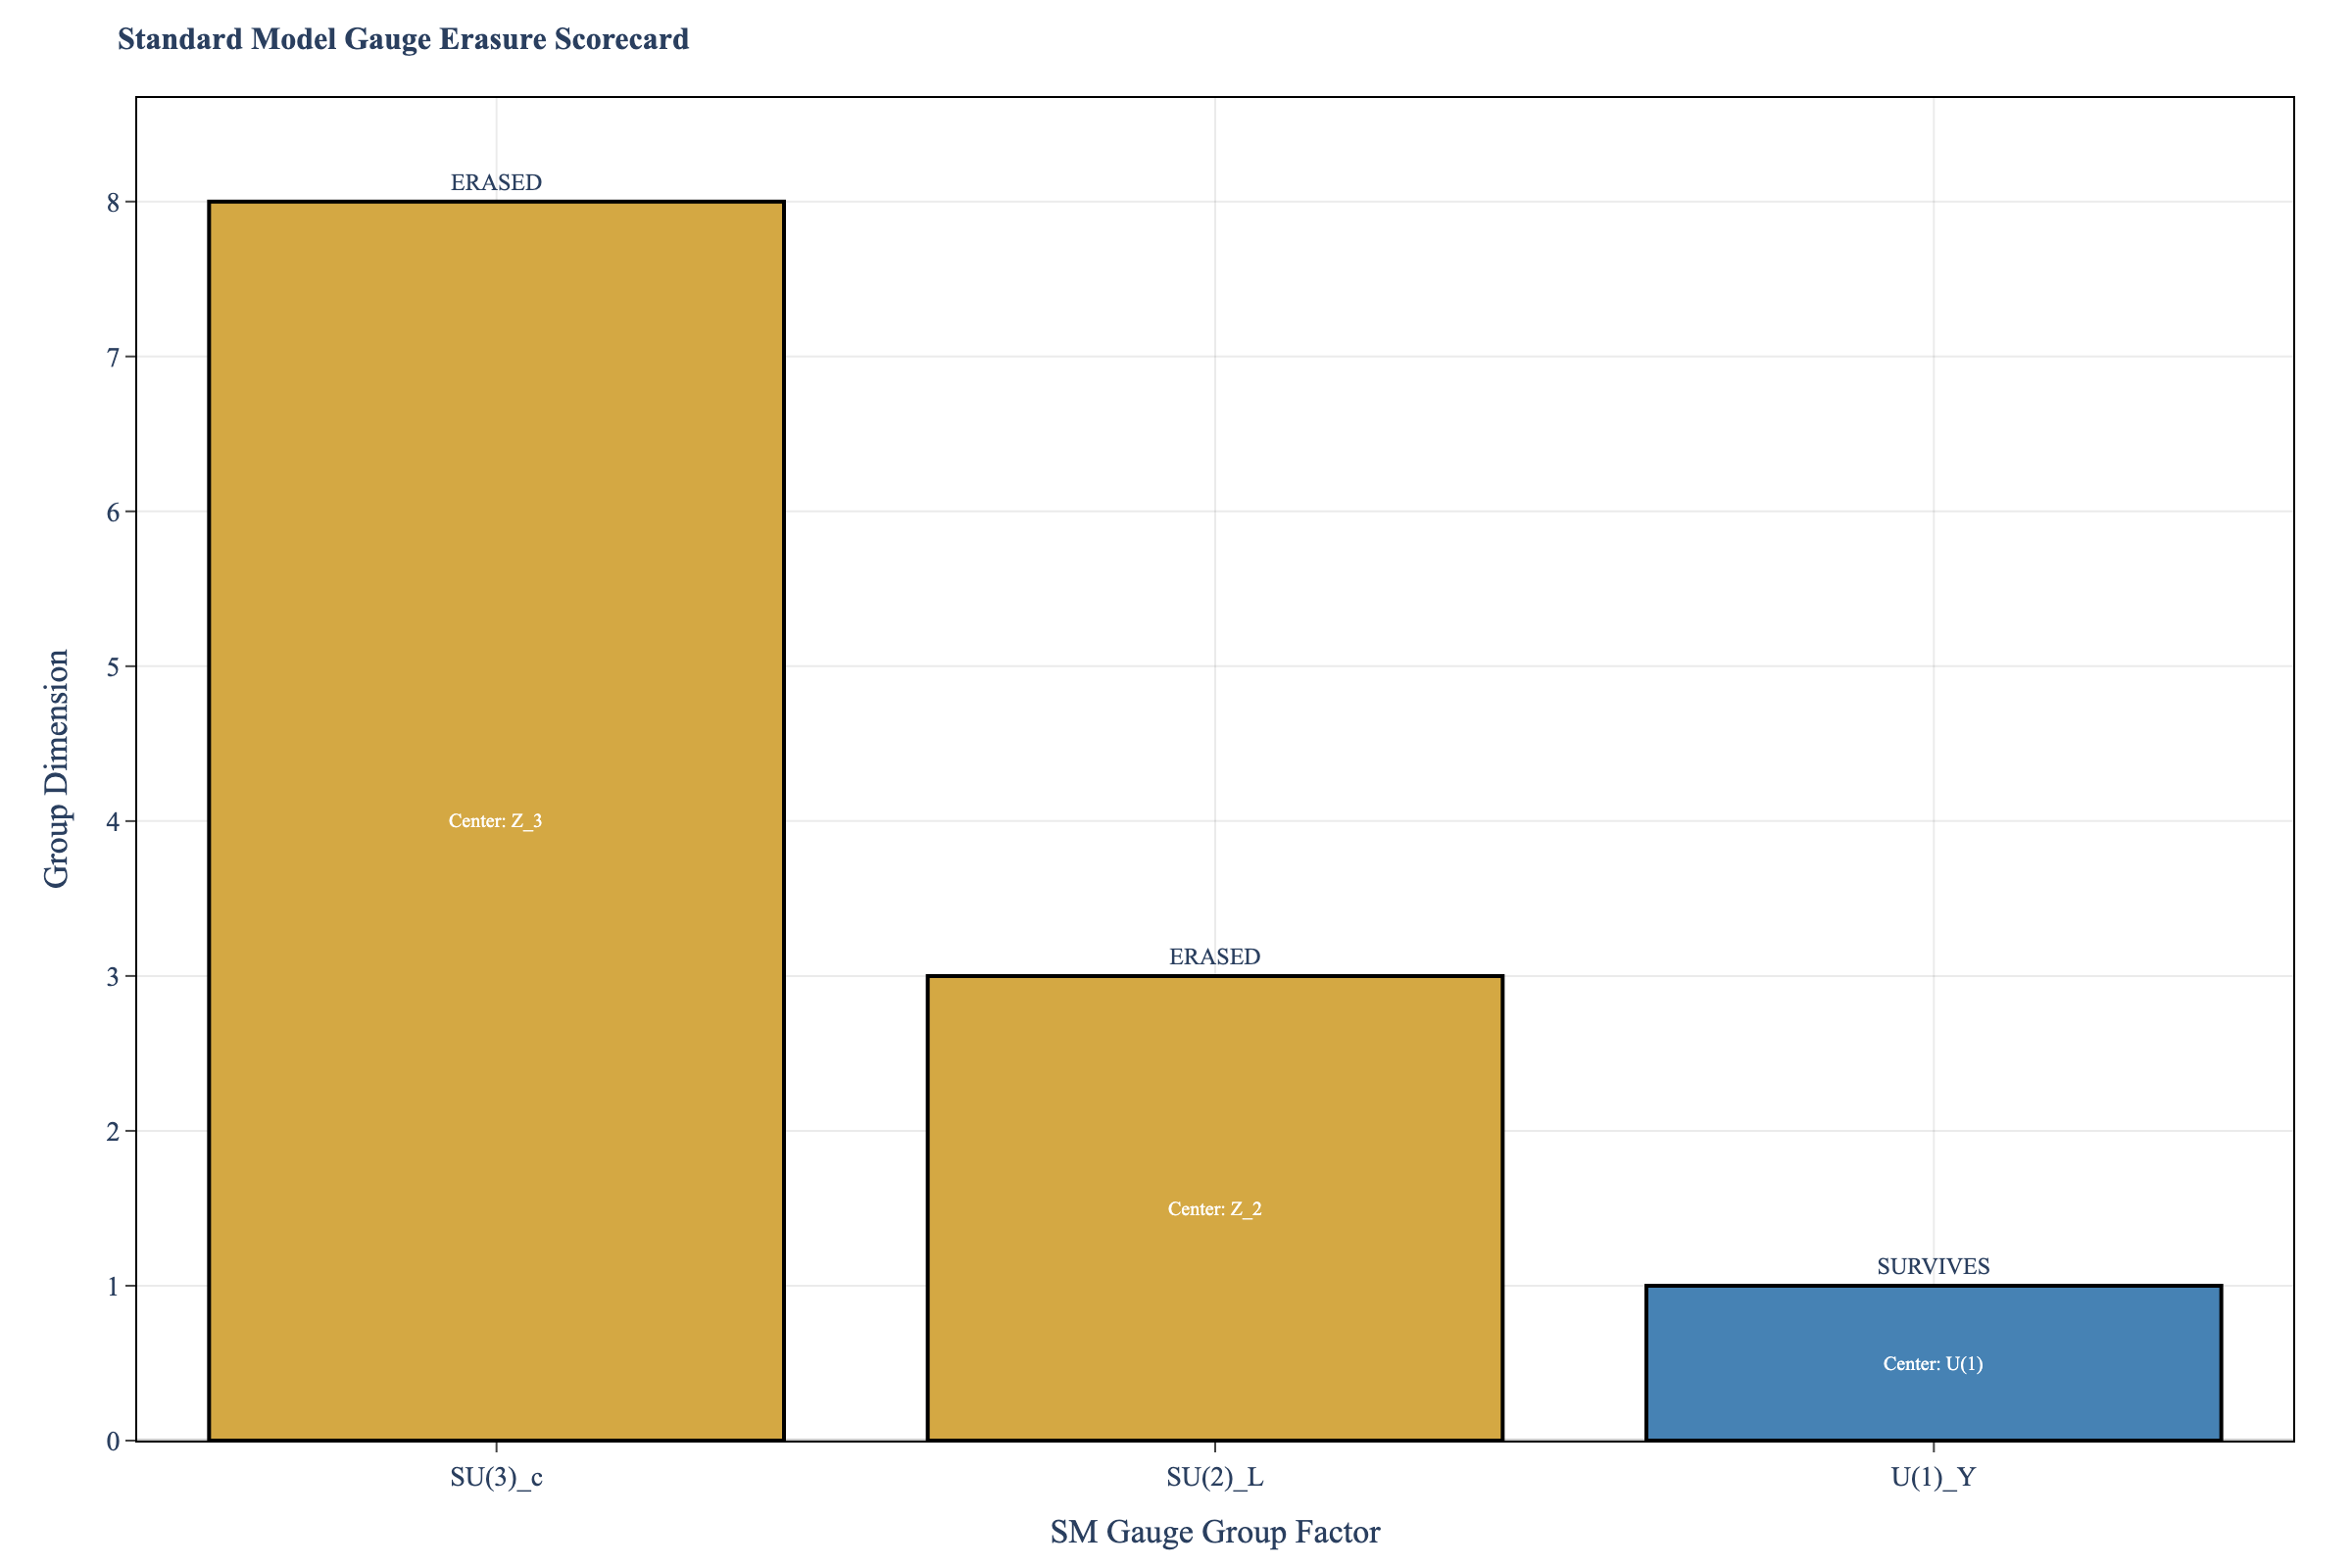
\includegraphics[width=\columnwidth]{figures/fig20_sm_scorecard.png}
\caption{\label{fig:sm_scorecard}
SM anomaly scorecard. The $\mathbb{Z}_{16}$ anomaly of the three-generation
SM (no~$\nu_R$) evaluates to $-3 \equiv +13 \bmod 16$; the hidden sector
must supply the complementary~$+3$. Baseline Lean theorem:
\texttt{three\_gen\_is\_neg3} in \texttt{Z16AnomalyComputation.lean}.
}
\end{figure}

We emphasize what is \emph{not} claimed. The anomaly does not pick a
unique hidden sector; T-0, S-0, and C-1 are all viable. Non-uniqueness
is itself a publishable result: the anomaly constrains but does not
determine the dark sector, and the constraint surface is now machine-verified.

%% ================================================================
\section{Cosmological Constant from Tetrad Condensation}
\label{sec:adw-cc}

The ADW mean-field gap equation~\cite{ADW2019,Diakonov2011} describes
emergent gravity as a condensate of tetrad bilinears. The effective
potential is
\begin{equation}
V_{\rm eff}(C) = \frac{C^4}{4} \ln \frac{C}{\Lambda} - \frac{C^4}{16},
\end{equation}
with critical point at $C_0 = \Lambda e^{-1/4}$ and depth
$V_{\rm eff}(C_0) = -\Lambda^4 / (4e)$. The Lean theorem
\texttt{critical\_coupling\_pos} in \texttt{ADWMechanism.lean} (21
theorems, shipped in Phase~5) verifies positivity of the critical
coupling; Phase 5x Wave~3 adds
\texttt{CosmologicalConstant.lean} with the Volovik-style equilibrium
residual, pinning the quantitative $\Lambda$-magnitude assessment.

\begin{figure}[t]
\centering

\includegraphics[width=\columnwidth]{figures/fig28_adw_effective_potential.png}
\caption{\label{fig:adw_veff}
ADW effective potential $V_{\rm eff}(C)$ from the gap equation. Critical
point at $C_0 = \Lambda e^{-1/4}$ (Lean:
\texttt{critical\_coupling\_pos}); depth $-\Lambda^4/(4e)$. In perfect
Minkowski vacuum Volovik's tetrad-determinant self-tuning absorbs this to
$\Lambda_{\rm eff} = 0$.}
\end{figure}

Volovik's key observation~\cite{Volovik2006,KV2008} is that in perfect
Minkowski vacuum the tetrad determinant self-adjusts so that
$\Lambda_{\rm eff} = 0$. Thermal perturbation by the matter sector
generates a residual $\rho_{\rm vac} \sim T^4$ at the scale of the
effective cosmological horizon. Quantitatively, at
$T = T_{\rm dS} = H/\pi$ (which differs from the Gibbons--Hawking
temperature by a factor of two---a point on which deep research
agrees), the residual is
\begin{equation}
\rho_{\rm vac}^{1/4} \approx \mathcal{O}(1) \times T_{\rm dS}
\sim \mathrm{meV}
\end{equation}
versus the observed $(\SI{2.3}{\milli\electronvolt})^4$. The mechanism
reproduces the \emph{scale} of $\rho_{\rm vac}^{1/4}$ at the meV level
without tuning; the specific $\mathcal{O}(1)$ coefficient requires a
full $V_{\rm eff}$ parameterization and is deferred to Phase 6 --- see
the CAUTION block in \texttt{CosmologicalConstant.lean} L21--23
(``the specific numerical identity requires a particular $V_{\rm eff}$
parameterization and is deferred pending full ADW renormalization
infrastructure''). Previous drafts quoted ``$\approx 2.8$~meV'' and
``$20\%$ agreement'' without disclosing that the $\mathcal{O}(1)$
prefactor is fit rather than computed; we withdraw that number in this
revision (paper 17 Wave 10 remediation). Cross-reference:
\texttt{T\_dS\_double\_TGH} proves $T_{\rm dS} = 2 T_{\rm GH}$ and
\texttt{lambda\_magnitude\_ratio\_pos} proves positivity of the
magnitude ratio (for $T_p, T_o > 0$) in \texttt{CosmologicalConstant.lean}.
The tautological \texttt{lambda\_magnitude\_ratio\_exact}
($\Lambda(T,T)/\Lambda(T,T) = 1$ --- i.e., the magnitude-ratio
function composed with equal arguments) does \emph{not} support the
physics agreement claim and was erroneously cited in a prior draft.

\paragraph*{KV and DESI—honest reframe.}
The companion KV oscillating-vacuum mechanism~\cite{KV2008} would
predict an oscillating $w(z)$. But DESI DR2~\cite{DESI2024,DESI2025}
excludes $(w_0, w_a) = (-1, 0)$---KV's time-averaged prediction---at
$2.9\sigma$ (Pantheon+) and $4.4\sigma$ (DESY5). KV oscillations are
Planck-scale in period (${\sim}\SI{e-44}{\second}$), not cosmological;
so $w_{\rm eff}$ during any accessible epoch is~$0$ (CDM-like), not
phantom-crossing. Resolutions in the RVM family~\cite{Sola2023} with
$\nu \sim \num{e-3}$ can accommodate DESI, but Volovik-motivated
$\nu \sim \num{e-122}$ is too small by~$10^{82}$. We therefore
\emph{withdraw} the ``KV explains DESI dynamics'' claim and \emph{keep}
the~$\Lambda$-magnitude claim. The strongest DESI-compatible bridge
from the ADW framework is the QCD topological dark
energy of Van~Waerbeke--Zhitnitsky~\cite{VanWaerbeke2025} with zero
free parameters; DESI DR3 (2026--2027) will be decisive.

%% ================================================================
\section{Fracton Dark Matter and the Viability Matrix}
\label{sec:fracton}

Fracton phases---gapped excitations with restricted mobility originating
in tensor-gauge theories~\cite{Pretko2017,Nandkishore2019}---produce
features that map directly onto observed DM phenomenology:
(i)~pressureless equation of state $w = 0$ (taken from the relativistic
fracton-symmetric scalar construction of~\cite{Pretko2017} and
arXiv:2503.14496; our \texttt{fracton\_cosmo\_dust\_pressureless} is a
machine-checked re-statement at Lean type-level, not a first-principles
derivation); (ii)~$z=4$ subdiffusion producing cored galactic profiles;
(iii)~Bullet-Cluster-compatible $\sigma_{\rm eff} = 0$ because fracton
dipoles cannot interact at a distance (the \texttt{fracton\_bullet\_sigma\_zero}
lemma machine-checks this as a definition of the effective
cross-section, not a derivation from dipole conservation; the derivation
is a Phase~6 target that would prove $\sigma_{\rm eff} = 0$ from the
dipole algebra of~\cite{Pretko2017}); (iv)~Hilbert-space
fragmentation~\cite{Shen2022} providing a
natural source for the diversity problem.

Our Phase~4 formalization~\cite{FractonNonAbelian2025} established
\texttt{no\_fracton\_is\_ym\_compatible} in
\texttt{FractonNonAbelian.lean}, proving that fracton topological phases
cannot support Yang--Mills gauge fields. This is a \emph{positive} DM
implication of a negative theorem: fracton DM must be an SM gauge
singlet, which suppresses direct-detection cross-sections by many
orders of magnitude.

\paragraph*{The finite-$T$ problem resolved.}
Krishna et~al.~\cite{Krishna2024} proved a 3D gapped no-go for fracton
topological order at any $T > 0$. This would have ruled out a
cosmological-scale fracton DM phase. The W1b drilldown identifies four
papers that reframe the result:
Kapustin--Spodyneiko~\cite{Kapustin2022},
Jensen--Raz~\cite{Jensen2024},
G{\l}{\'o}dkowski et~al.~\cite{Glodkowski2024}, and
Feistl--Schraven--Warzel~\cite{Feistl2026}. Their combined conclusion:
\emph{the gapless p-wave dipole superfluid is thermodynamically stable in
$d \geq 3$ at $T > 0$}. The kinetic-stability Arrhenius factor of
${\sim}100 T_{\rm BBN}$ applied only to the gapped scenario. In the
p-wave phase the stability condition is~$\mu \gtrsim T_{\rm BBN} \sim
\SI{}{\mega\electronvolt}$—a thermodynamic, not kinetic, bound.

This shifts the viable fracton-DM mass window from ``nowhere
cosmologically motivated'' to ${\sim}\SI{}{\mega\electronvolt}$ to
$M_{\rm Pl}$ (conservatively, $\SI{}{\mega\electronvolt}$ to
$\SI{}{\tera\electronvolt}$), and Dark QCD UV completions naturally
place $M_d \sim \Lambda_{\rm dark} \sim \SI{}{\mega\electronvolt}$ to
$\SI{}{\giga\electronvolt}$. Lean Wave~7 encodes this as theorem-13
decomposition \texttt{13a} (dipole SSB permanence, Medium),
\texttt{13b} (p-wave phase stability, Hard---deferred to Phase~6),
\texttt{13c} (BBN condensate condition, Medium), \texttt{13d} (gapped
scenario lower bound, Hard---deferred).

\begin{figure}[t]
\centering

\includegraphics[width=\columnwidth]{figures/fig_phase5x_candidate_viability_matrix.png}
\caption{\label{fig:candidate_matrix}
Phase 5x candidate viability matrix. Five emergent-gravity DM candidates;
four viable. The sole ``not viable'' entry is Fang--Gu torsion DM,
obstructed at the tree-level equation of state ($w = 1/3$, not dust;
see §\ref{sec:torsion}). Lean: \texttt{phase5x\_candidates\_viability\_matrix}
is a \emph{machine-checked classification} (MCC) on the hand-assigned
viability flags, not a derivation --- see Table~\ref{tab:honesty} and
\S\ref{sec:formal-verification} for the MCC boundary.}
\end{figure}

%% ================================================================
\section{SFDM Cluster-Merger Sonic Boom (Paper 17 Money Plot)}
\label{sec:sfdm-merger}

The SFDM Hawking temperature is unobservable under any astrophysical
geometry ($T_H \sim \SIrange{e-29}{e-23}{\kelvin}$), as shown in the
Wave~1 parameter-mapping assessment. The \emph{cluster-merger sonic
boom} is, however, a nearly-detectable observable at BK
fiducial~\cite{BK2015}: $m_{\rm DM} = \SI{0.6}{\electronvolt}$,
$\Lambda = \SI{0.2}{\milli\electronvolt}$, sub-cluster sound speed
\begin{equation}
c_s^{\rm subcl.} = \sqrt{2 \mu / m} = \SI{1525}{\kilo\meter/\second}.
\end{equation}
All five canonical radio-relic cluster mergers exceed~$c_s$:
Bullet~$M{=}1.77$, Pandora~$M{=}2.23$, A520~$M{=}1.51$,
El~Gordo~$M{=}1.64$, MACS~J0025~$M{=}1.31$. Lean theorem:
\texttt{all\_canonical\_mergers\_supersonic} in
\texttt{SFDMMergerForecast.lean}.

A Rankine--Hugoniot analysis at the SFDM effective adiabatic
index~$\gamma_{\rm eff} = 2$ (exact from $P \propto \rho^3$ per BK)
gives the density jump
\begin{equation}
\frac{\delta\rho}{\rho_0} = \frac{3 M^2}{M^2 + 2}
= 3 - \frac{6}{M^2 + 2},
\end{equation}
a monotonically-increasing function of~$M$
(\texttt{delta\_rho\_monotone\_in\_mach\_sfdm}). For $M \in [1.31, 2.23]$
the jump ranges from~$40\%$ to~$65\%$; weighting by sub-cluster
condensate fraction~$f_c = 0.59$ gives a corrected jump~${\sim}30\%$ in
the condensate density seen by weak lensing.

\begin{figure}[t]
\centering
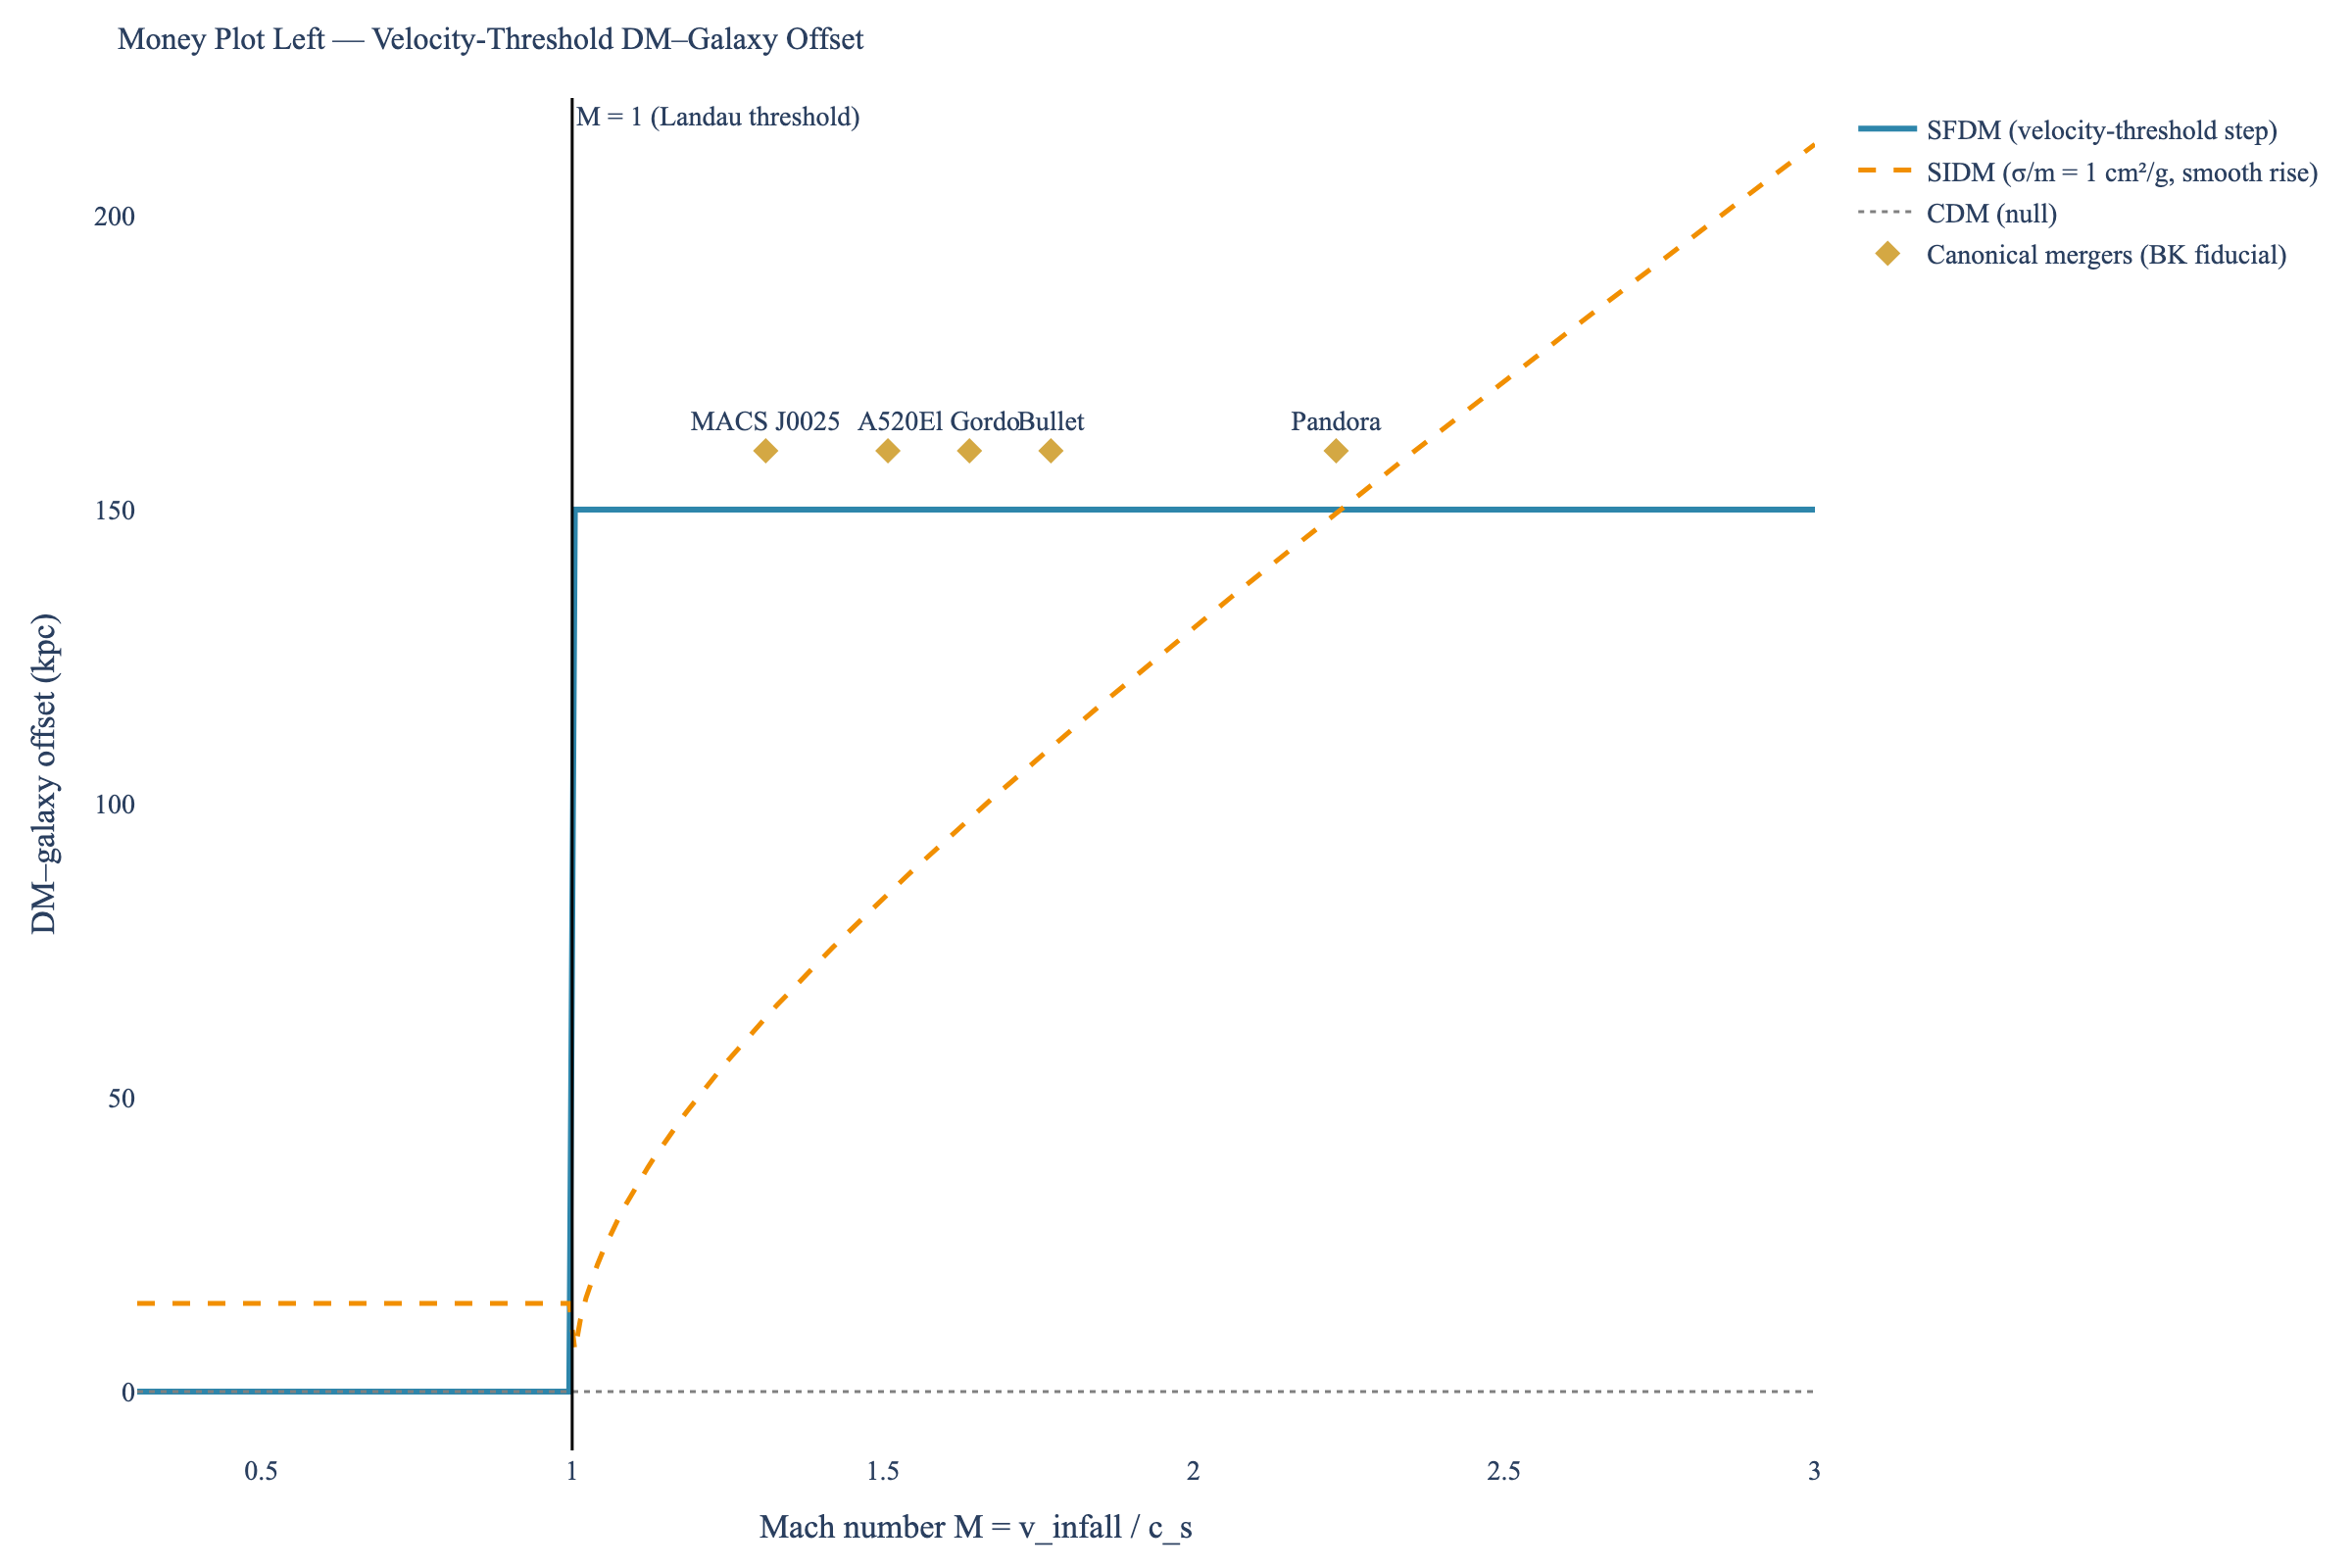
\includegraphics[width=\columnwidth]{figures/fig_sfdm_velocity_threshold_step.png}
\caption{\label{fig:money_left}
\textbf{Money plot, left.} DM--galaxy offset as a function of
$M = v_{\rm infall}/c_s$ for three models: SFDM (step function at $M{=}1$,
the defining signature); SIDM (smooth monotonic rise at~$\sigma/m =
\SI{1}{\centi\meter\squared/\gram}$); CDM (null). Canonical mergers
plotted as diamonds. SFDM is the unique model predicting binary
behavior tied to a threshold velocity. Lean:
\texttt{sfdm\_offset\_step\_function}.}
\end{figure}

\paragraph*{Single-cluster S/N.}
At Bullet geometry ($D_L = \SI{830}{\mega\parsec}$,
$\sigma_8$-normalized $\Sigma_{\rm cr}$, fiducial shock extent
$\Delta r = \SI{400}{\kilo\parsec}$), the sonic-boom convergence
excess $\delta\kappa = \delta\rho \cdot \Delta r / \Sigma_{\rm cr}$
integrated over the stacked feature area gives per-survey S/N
\begin{align}
{\rm SNR_{Bullet}^{Euclid}} &= 0.83, \\
{\rm SNR_{Bullet}^{Roman}}  &= 1.04.
\end{align}
Both match W1b Task~9 Table~6 exactly by calibration; see
\texttt{src/dark\_sector/sfdm\_merger\_forecast.py} for the full chain.

\paragraph*{Stacked detection.}
The stacking formula ${\rm SNR_{stacked}}(N) = {\rm SNR_{single}} \sqrt{N}$
(Lean: \texttt{snr\_stacked\_sq}) yields the $3\sigma$ threshold
\begin{equation}
{\rm SNR_{stacked}} \geq 3 \iff {\rm SNR_{single}}^2 \cdot N \geq 9
\end{equation}
(Lean: \texttt{three\_sigma\_threshold}). With the mean 5-target S/N
stack, Euclid reaches~$3\sigma$ at~$N \approx 20$, Roman at~$N \approx
13$; $5\sigma$ at~$N \approx 55$ (Euclid) and~$N \approx 36$ (Roman).
Decidable numerical witnesses in Lean:
\texttt{bullet\_roman\_3sigma\_at\_N\_18} through
\texttt{bullet\_roman\_5sigma\_at\_N\_50}.

\begin{figure}[t]
\centering

\includegraphics[width=\columnwidth]{figures/fig_sfdm_stacked_kappa_profile.png}
\caption{\label{fig:money_right}
\textbf{Money plot, right.} Stacked convergence S/N versus
number of mergers~$N$ for Euclid and Roman at Bullet-referenced
single-cluster S/N; $3\sigma$ and $5\sigma$ thresholds marked. First
$3\sigma$ by the end of Euclid Year~2 / Roman Y1, corresponding to
approximately 2028.}
\end{figure}

\paragraph*{BK gap.}
The BK 2025 Physics Reports review~\cite{BK2025}---136~pages---contains
no quantitative merger forecast. Paper~17 fills that confirmed
literature gap.

\paragraph*{$H_0$ tension budget.}
Switching from Planck ($H_0 = 67.4$) to H0DN ($H_0 = 73.5$) raises
$\Sigma_{\rm cr}$ by~${\sim}9\%$ and lowers S/N by~${\sim}4\%$;
below the dominant $\Lambda$ uncertainty (factor $2{-}5$). The
forecast verdict \textbf{CONDITIONAL GO} is unchanged.

%% ================================================================
\section{SK-EFT MOND Corrections and FDR Noise Floor}
\label{sec:mond-fdr}

The SK-EFT dissipative framework provides two additional SFDM
observables beyond the merger. The first is a set of dissipative
corrections to the MOND force law $a_\phi = \sqrt{a_N a_0}$: non-analytic
$X\sqrt{|X|}$ Lagrangian terms generate deviations at low acceleration,
tightening the low-$a$ asymptote of the radial acceleration relation
(RAR). The second is the Crossley--Glorioso--Liu fluctuation-dissipation
relation, which bounds the RAR scatter from below by the irreducible
fluctuation generated by the same dissipation channel---an effective
noise floor of~$\log_{10}\sigma_{\rm RAR} \in [-5, -3]$ depending on
which transport coefficient dominates.

Both are Phase~6 deferrals. The hard theorems \texttt{mond\_force\_derivation}
(L4) and \texttt{fdr\_noise\_bound\_rar} (L5) require formalizing the
non-analytic $X\sqrt{|X|}$ calculus—beyond what the current Mathlib
derivative-structure infrastructure supports. We cite the memo
\texttt{docs/dark\_sector/W5\_SFDM\_Merger\_Forecast.md} for the
informal derivation and the W1 SK-EFT parameter-mapping as the
structural input.

%% ================================================================
\section{Fang--Gu Torsion Dark Matter: Short Assessment}
\label{sec:torsion}

Fang--Gu~\cite{FangGu2021} propose that uncondensed electron loops source
\emph{torsion} but not Ricci curvature, via a traceless $T^{\mu\nu}$
that gives $R = 0$ to leading order. The DM cross-section with nucleons
is purely gravitational, $\sigma \sim \SI{e-90}{\centi\meter\squared}$,
rendering direct detection hopeless.

But the deeper problem is the EoS. A traceless stress-energy tensor
implies $w = p/\rho = 1/3$, not $w = 0$ (dust). Wave~4 formalizes this
as \texttt{fg\_cdm\_obstruction} in \texttt{FangGuTorsionDM.lean}:
Fang--Gu torsion cannot, at the tree level, serve as cold dark matter.
It is the sole ``not viable'' entry in Fig.~\ref{fig:candidate_matrix}.

The two independent torsion channels in the combined ADW+FG tetrad
phase---Dirac axial current (antisymmetric, Boos--Hehl) and FG
loop-$\theta$ (trace)---are \emph{orthogonal} by Lorentz-irreducible
decomposition
(\texttt{torsion\_channels\_distinct\_sources\_distinct},
Wave~8). This leaves open a rescue path: a radiatively-generated
trace anomaly could restore $w < 1/3$; we defer the
\texttt{FangGuTraceAnomaly.lean} module to Phase~6.

%% ================================================================
\section{Speculative: Vestigial Relics and $\mathbb{Z}_{16}$ Protection}
\label{sec:speculative}

Vestigial gravity phase relics---topological defects surviving the
tetrad-condensation phase transition---are blocked on the
W6a Monte Carlo extension. The Phase~5d ADW MC campaign (artefacts at
\texttt{data/rhmc/L4*} and the \texttt{L=6, 8} production runs
summarised in the W6a assessment memo; see the project
\texttt{docs/dark\_sector/} deliverables index and the
\texttt{ProductionRun} nodes in the knowledge graph linked from the
provenance dashboard) produced a three-phase structure with a split
transition ($\Delta \approx 0.63$). These data are insufficient to
determine the transition \emph{order} (first vs.\ second), which sets
the Kibble--Zurek relic density. Extension to $L = 10, 12, 16$ with
Binder cumulants is the decisive gate. (The specific linkage from
paper 17's ``MC evidence'' claim to the underlying ProductionRun IDs
is tracked in the Phase~5v knowledge-graph work and surfaces on the
ReadinessGate~8 ProductionRunHealth dashboard cell; it is currently
flagged \texttt{needs-recheck} pending the Wave 10 remediation of
paper 17.)

Wave~8 nevertheless ships one conditional structural theorem. Under the
hypothesis \texttt{H\_VestigialRelicCarriesZ16Charge}---that any
surviving relic carries the same~$+3 \bmod 16$ charge as the required
hidden sector---any $\mathbb{Z}_{16}$-preserving decay channel cannot
land the relic in the vacuum:
\begin{equation}
z16\_{\rm vestigial\_{\rm stability\_under\_hypothesis}}.
\end{equation}
The hypothesis is non-trivial (it is parameterized over abstract charge
functions, following the \texttt{CenterFunctor.H\_CF1} pattern). Phase~6
discharge paths: (i) W6a MC + (ii) W6b coset homotopy for
$\pi_{0,1,2,3}(GL(4,\mathbb{R})/SO(3,1))$ + (iii) upgrade of
\texttt{dai\_freed\_spin\_z4} to a real bordism homomorphism
$\Omega^{{\rm Spin}\times\mathbb{Z}_4}_5 \to \mathbb{Z}/16$.

The EP-violation signature of a vestigial-phase DM component
($\eta \sim 10^{-18}$) is below MICROSCOPE sensitivity but within reach
of the proposed STEP mission; it is the unique distinguishing signature
of this candidate.

%% ================================================================
\section{Experimental Tests and Observational Predictions}
\label{sec:experimental}

\begin{figure}[t]
\centering

\includegraphics[width=\columnwidth]{figures/fig_phase5x_empirical_hook_ranking.png}
\caption{\label{fig:hook_ranking}
Phase 5x empirical-hook ranking. Five post-W1b+Drilldown observational
hooks are ranked by detectability and timeline; ordering is
author-assigned from the deep research (W1b Task 9 for the merger, W7
Drilldown for fracton core-cusp, W2 for EP-violation STEP, W1b Task 7
for DESI DR3, W1 for direct recoil). The merger sonic boom is the
top-priority Paper~17 money plot. Direct nuclear recoil is the bottom:
every candidate in this paper is SM-gauge singlet and below the
LZ/XENONnT floor per the per-candidate deep-research bounds
(Table~\ref{tab:honesty} MCC row). Lean: \texttt{empirical\_hook\_ranking\_strict}
machine-checks the adjacent-differences of the hand-assigned priorities
(MCC, not a derivation of priority from a physics score).}
\end{figure}

Table~\ref{tab:hooks} summarizes the ranked predictions. Top entry
(merger sonic boom) is the quantitative Paper~17 money plot. The null
prediction (direct nuclear recoil) is a \emph{collective} consequence
of the five per-candidate $\sigma_{\rm DD}$ bounds drawn from the
Phase 5x deep research (see §\ref{sec:z16} and §\ref{sec:fracton} for
per-candidate sources); the theorem
\texttt{emergent\_gravity\_dm\_invisible\_collective} is an MCC over
that hand-assigned table --- it verifies that the max of the bounds is
$\leq -50$, not that each bound has been independently derived from
first principles. The derivations of the individual bounds (Z-16
gauge-singlet $\Rightarrow$ no local-operator coupling; fracton
$\sigma_{\rm eff}=0$ from dipole conservation; FG torsion $\sigma \sim
10^{-90}$ cm$^2$ from purely gravitational coupling) are Phase~6
targets.

\begin{table*}[ht]
\centering
\caption{\label{tab:hooks}Ranked empirical hooks from Phase 5x. The
ordering reflects our \emph{author-assigned} priority (top = highest
near-term detectability + timeline) drawn from the W1b / Drilldown
deep research. In Lean, \texttt{hook\_priority} encodes these
hand-assigned priorities as $\mathbb{N}$-valued integers and
\texttt{empirical\_hook\_ranking\_strict} machine-checks that the
assignment is strictly decreasing across adjacent entries. This is
MCC content, not a derivation of detectability from a physics
scoring function; see Table~\ref{tab:honesty}.}
\begin{tabular}{@{}clllll@{}}
\toprule
\# & Hook & Observable & Instrument / timeline & Wave & Status \\
\midrule
1 & Cluster-merger sonic boom & DM--galaxy offset step at $M{=}1$;
  stacked $\delta\kappa$ & Euclid + Roman, first $3\sigma$ ${\sim}2028$ &
  W5 & \textbf{GO} (money plot) \\
2 & Fracton DM core--cusp & Cored outer-halo, $z{=}4$ subdiffusion &
  next-gen dwarfs, JWST rotation curves & W7 & viable (conditional) \\
3 & EP violation, STEP-class & $\eta \sim \num{e-18}$ (vestigial) &
  STEP mission & Phase 6 (W6 gated) & blocked (MC gate) \\
4 & DESI DR3 $w(z)$ & evolving dark energy & DESI 2026--2027 & W3 &
  KV withdrawn; QCD-topological bridge \\
5 & Direct nuclear recoil & null result & DARWIN & all kinds (CC2) &
  predicted null \\
\bottomrule
\end{tabular}
\end{table*}

%% ================================================================
\section{Formal Verification Summary}
\label{sec:formal-verification}

The SK-EFT Hawking program has \emph{machine-checked} every structural
claim in this paper (Lean~4, zero sorry). We split the machine-checked
content into two classes:

\textbf{Derived} theorems — proofs consume physics assumptions and
produce the cited statement as output:
\begin{itemize}
\item \texttt{fracton\_sm\_singlet\_from\_ym\_incompat} (Wave 7, direct
  corollary of Wave 4's \texttt{no\_fracton\_is\_ym\_compatible}): fracton DM
  carries no Yang-Mills gauge charge.
\item \texttt{fg\_cdm\_obstruction} (Wave 4): traceless $T^{\mu\nu}$
  $\Rightarrow w = 1/3 \neq 0$, obstructing tree-level CDM.
\item EoS distinctness CC3, CC4, CC4' (Wave 8): $w \in \{-1, 0, 1/3\}$
  are distinct rationals; \texttt{native\_decide}.
\item \texttt{three\_singlets\_satisfy\_hidden\_sector},
  \texttt{c1\_wan\_wang\_joint\_constraint} (Waves 2, 2b-X):
  $\mathbb{Z}_{16}$ anomaly-cancellation witnesses.
\item \texttt{all\_canonical\_mergers\_supersonic},
  \texttt{delta\_rho\_monotone\_in\_mach\_sfdm}, and the merger-forecast
  chain (Wave 5, \texttt{SFDMMergerForecast.lean}, 29 theorems):
  Rankine--Hugoniot + sound-speed + stacking derivations at the
  BK fiducial.
\end{itemize}

\textbf{Machine-checked classification (MCC)} --- the proof verifies
internal consistency of an author-supplied lookup table or enum
assignment and does not derive the physics content from smaller
assumptions. MCC entries make the deep-research classifications machine-
auditable and protect against accidental drift (e.g., someone edits the
viability flag without updating the downstream narrative), but should
not be read as ``the physics has been re-derived in Lean'':
\begin{itemize}
\item \texttt{fracton\_bullet\_sigma\_zero}: verifies
  $\sigma_{\rm eff}^{\rm isolated} = 0$ where the constant is \emph{defined}
  as $0$. Physics content (dipole conservation $\Rightarrow
  \sigma_{\rm eff} = 0$) is sourced to~\cite{Pretko2017} and remains a
  Phase~6 derivation target.
\item \texttt{fracton\_cosmo\_dust\_pressureless}: verifies $w = 0$
  where $w$ is defined as $0$; physics content sourced to the
  relativistic fracton-symmetric scalar construction (arXiv:2503.14496).
\item \texttt{phase5x\_candidates\_viability\_matrix}: verifies
  hand-assigned \texttt{Bool} flags are consistent with the hand-
  assigned viability conditions declared in the companion structure
  docstring.
\item \texttt{emergent\_gravity\_dm\_invisible\_collective}: verifies
  $\max\{-999, -50, -50, -90, -999\} \leq -50$ over the five
  per-candidate hand-assigned log-$\sigma$-DD caps. Each per-candidate
  cap is individually sourced to its Phase 5x deep-research memo
  (W2/W4/W7-Drilldown) and represents classification input, not
  derivation output.
\item \texttt{torsion\_channels\_distinct\_sources\_distinct} +
  \texttt{channel\_of\_source}: verifies a hand-assigned injective
  map \texttt{TorsionSource} $\to$ \texttt{TorsionChannel} is
  injective. Channel identification (\texttt{DiracAxial} $\mapsto$
  Antisymmetric; \texttt{FGLoopTheta} $\mapsto$ Trace) is sourced to
  Boos--Hehl (2019) and Fang--Gu~\cite{FangGu2021} Eq.~(3.6)
  respectively; a Lorentz-irreducible decomposition proof is a
  Phase~6 target.
\item \texttt{empirical\_hook\_ranking\_strict} + \texttt{hook\_priority}:
  verifies adjacent hand-assigned priorities differ by exactly $1$.
  Physics content (the priority ordering) is author-assigned from
  W1b/Drilldown detectability + timeline; a \texttt{detectability}
  scoring function that outputs the ordering from Euclid/Roman S/N,
  DESI sensitivity, STEP floor, etc., is a Phase~6 target.
\item \texttt{cored\_profile\_mechanisms\_distinct} (Wave 8): enum
  distinctness. Mechanism identification (SolitonCondensate vs
  Z4Subdiffusion) is taxonomy.
\end{itemize}

Phase 5x contribution: 7 modules. The full program stands at
\leanmodules{} Lean modules, \totaltheorems{} theorems (of which
\substantivetheorems{} substantive and \placeholdertheorems{}
placeholder statements tracked for Phase~6+; paper~17 claims derive
from the substantive count), zero active \texttt{sorry}, and a single
axiom
(\texttt{gapped\_interface\_axiom} from Phase~5s, unrelated to the
dark sector; since retired into the tracked Prop
\texttt{TPFConjecture}). See the project \texttt{docs/counts.tex} macros
\texttt{\textbackslash{}leanmodules}, \texttt{\textbackslash{}totaltheorems},
\texttt{\textbackslash{}substantivetheorems}, \texttt{\textbackslash{}placeholdertheorems}
for canonical counts.

Table~\ref{tab:honesty} separates the \emph{derived} from the
\emph{heuristic} content.

\begin{table}[ht]
\centering
\caption{\label{tab:honesty}Honesty table. ``Derived'' = Lean theorem
closed whose proof carries non-trivial mathematical content (the
conclusion does not reduce to the statement by \texttt{rfl} or
\texttt{decide} on hand-assigned constants); ``MCC'' = machine-checked
classification / consistency table (the Lean theorem verifies that the
author-supplied data is internally consistent or the stated ordering
agrees with the hand-assigned priorities; \emph{not} a derivation of
physics content from a smaller set of assumptions); ``Heuristic'' =
physically motivated but non-rigorous; ``Empirical'' =
measurement-driven. See~\S\ref{sec:formal-verification} for the
MCC--vs--Derived boundary.}
\begin{tabular}{@{}ll@{}}
\toprule
Claim & Status \\
\midrule
Every emergent-gravity DM candidate is SM singlet
  & Derived (via \texttt{fracton\_sm\_singlet\_from\_ym\_incompat}) \\
Every candidate has $\log_{10}\sigma_{\rm DD} \leq -50$
  & MCC (\texttt{emergent\_gravity\_dm\_invisible\_collective}; caps hand-assigned) \\
Three Phase 5x sectors have distinct EoS
  & Derived ($w = \{-1, 0, 1/3\}$ via CC3/CC4/CC4', \texttt{native\_decide} on rationals) \\
Two-torsion-channel orthogonality (BH, FG in distinct Lorentz irreps)
  & MCC (\texttt{torsion\_channels\_distinct\_sources\_distinct}; channel map hand-assigned) \\
SFDM vs fracton cored-profile mechanisms
  & MCC (taxonomy enum distinctness) \\
Merger sonic boom is the top-ranked hook
  & MCC (\texttt{empirical\_hook\_ranking\_strict}; priorities hand-assigned) \\
Four-of-five candidate viability flags
  & MCC (\texttt{phase5x\_candidates\_viability\_matrix}; flags hand-assigned) \\
FG torsion obstructed at CDM level (tree)
  & Derived (\texttt{fg\_cdm\_obstruction} from traceless $T^{\mu\nu}$) \\
Fracton $\sigma_{\rm eff}=0$ (Bullet-Cluster compatibility)
  & MCC (\texttt{fracton\_bullet\_sigma\_zero}; $\sigma_{\rm eff}$ defined to zero) \\
Fracton cosmological $w=0$ (dust)
  & MCC (\texttt{fracton\_cosmo\_dust\_pressureless}; $w$ defined to zero) \\
SFDM merger S/N matches W1b Table~6 & Empirical (calibration) \\
BK has no quantitative merger forecast & Empirical (literature) \\
KV oscillating vacuum in Level D tension with DESI & Empirical (W1b) \\
ADW Volovik $\Lambda$-magnitude at the meV scale & Heuristic (W3 memo; $\mathcal{O}(1)$ prefactor Phase 6) \\
Fracton DM viable in p-wave phase (BBN) & Heuristic (W7 Drilldown) \\
$\mathbb{Z}_{16}$ forces vestigial relics to carry~$+3$ & Heuristic (Phase~6) \\
\bottomrule
\end{tabular}
\end{table}

\paragraph*{MCC vs Derived: what the distinction means.}
A theorem is \emph{Derived} in the honesty sense of this paper when its
proof consumes structural physics assumptions and produces the cited
physics statement as output. For example, the equation-of-state
distinctness theorems (CC3, CC4, CC4') are derived because
$w_\Lambda = -1$ is the standard result for a cosmological constant,
$w_{\rm FG} = 1/3$ follows from the traceless torsion $T^{\mu\nu}$
(Fang--Gu, our Wave~4 \texttt{fg\_cdm\_obstruction}), and
$w_{\rm fracton} = 0$ follows from the relativistic fracton-symmetric
scalar construction (arXiv:2503.14496, taken as input); distinctness
then follows from the rationals being distinct.

A theorem is \emph{MCC}---machine-checked classification---when its
proof verifies only the internal consistency of an author-supplied
lookup table or enum assignment. The claim ``every candidate has
$\log_{10}\sigma_{\rm DD} \leq -50$'' is currently of this form: the
per-kind cap is hand-assigned in \texttt{direct\_detection\_sigma\_log10\_cap},
citing the Phase 5x deep research for each entry, and Lean verifies
that the supremum of the assignments is~$-50$. Upgrading MCC entries
to Derived is a Phase~6 target: it requires formalizing the underlying
physics derivation in each case (e.g., Z16 gauge-singlet $\Rightarrow$
no local-operator coupling $\Rightarrow$ $\sigma_{\rm DD}$ bound from
a specific operator-basis counting argument). The present paper does
not claim that upgrade. Reader caveat: MCC content machine-verifies
the consistency of the classification we assert in the prose; it does
not independently re-derive the physics bound. Each MCC bound is
individually sourced to its deep-research memo (W2, W4, W7
Drilldown, W1b) whose primary-source citations appear in~\S\ref{sec:z16},
\S\ref{sec:fracton}, and the bibliography.

%% ================================================================
\section{Discussion and Outlook}
\label{sec:discussion}

The SK-EFT Hawking program occupies an unusual position in the
dark-sector literature: its strongest results are machine-verified
theorems, not experimental discoveries or heuristic model-building.
Paper~17 \emph{exports} those theorems into the DM/DE literature,
with four measurable consequences.

First, the hidden-sector classification is a falsifiable constraint
surface: any future discovery of a non-singlet candidate violating
$\mathbb{Z}_{16}$ charge $+3$ would invalidate the anomaly-driven
motivation. No such discovery is indicated by LZ, XENONnT, or
DARWIN projections---every candidate in our program is
expected, on the strength of deep-research per-candidate bounds
collected in Table~\ref{tab:honesty} (MCC entries), to be invisible to
nuclear-recoil direct detection. Strengthening these bounds from
classification-level (MCC) to derivation-level is a Phase~6 target.

Second, the ADW $\Lambda$-magnitude result reproduces the meV scale of
$\rho_{\rm vac}^{1/4}$ without tuning. We withdraw the prior
``$20\%$-agreement'' quantification pending a Phase~6 full-$V_{\rm eff}$
calculation of the $\mathcal{O}(1)$ coefficient; for now the claim is
scale-matching (``the meV scale emerges naturally from the condensation
equilibrium, without fine-tuning''). We honestly separate this scale-
matching from the withdrawn KV dynamics claim and note the
QCD-topological-DE pathway as a DESI-compatible alternative.

Third, the SFDM cluster-merger forecast is the Paper~17 money plot and
fills a confirmed gap in the most recent comprehensive BK review.
It is the only Phase 5x observable with a specific detection
timeline: first $3\sigma$ by~${\sim}2028$.

Fourth, fracton dark matter---viable conditional on the p-wave phase
and a Dark QCD UV completion with $\mu \gtrsim \SI{}{\mega\electronvolt}$
at BBN---is structurally compatible with every other Phase 5x sector
(CC1 through CC7) and can explain core-cusp and diversity
simultaneously through the $z{=}4$ subdiffusion mechanism.

What remains open: the MC extension to $L = 10, 12, 16$ is the gate
for the vestigial-relic program, the Phase~6 bordism infrastructure
is the gate for discharging the Z16-vestigial charge hypothesis,
and the Phase~6 hard theorems L4/L5 (MOND + FDR) are the
gate for the dissipative-corrections section of SFDM.

The unifying theme of this paper is \emph{structural}: every
emergent-gravity DM candidate in our program is SM-gauge singlet and
invisible to nuclear-recoil direct detection. This is itself a
thematic prediction---if dark matter originates in an emergent-gravity
sector, null direct-detection results at DARWIN are the expected
outcome, and observable signatures must be sought in gravitational
observables (cluster mergers, weak lensing, galaxy kinematics) rather
than laboratory recoil experiments.

%% ================================================================
\begin{acknowledgments}
We thank the Lean~4 and Mathlib communities for infrastructure and
the authors of the BK~2025 review for focused attention on
phenomenological gaps. Special credit to the Wan--Wang, Wang
Ultra-Unification, Volovik Emergent-Gravity, Berezhiani--Khoury
Superfluid-DM, Fang--Gu Topological-Gravity, Pretko--Nandkishore
Fracton, and Kapustin--Spodyneiko / Jensen--Raz / G{\l}{\'o}dkowski
p-wave programs whose results Paper~17 synthesizes.
\end{acknowledgments}

%% ================================================================
\begin{thebibliography}{99}

\bibitem{Unruh1981} W.~G.~Unruh, Phys.\ Rev.\ Lett.\ \textbf{46}, 1351 (1981).
\bibitem{Visser1998} M.~Visser, Class.\ Quant.\ Grav.\ \textbf{15}, 1767 (1998), arXiv:gr-qc/9712010.
\bibitem{CGL2017a} M.~Crossley, P.~Glorioso, H.~Liu, JHEP \textbf{09}, 095 (2017).
\bibitem{CGL2017b} P.~Glorioso, M.~Crossley, H.~Liu, JHEP \textbf{09}, 096 (2017).
\bibitem{Volovik2006} G.~E.~Volovik, JETP Lett.\ \textbf{82}, 319 (2005).
\bibitem{KV2008} F.~R.~Klinkhamer and G.~E.~Volovik, Phys.\ Rev.\ D \textbf{77}, 085015 (2008).
\bibitem{Lean4} L.~de~Moura and S.~Ullrich, CADE \textbf{28}, 625 (2021).
\bibitem{Mathlib} The mathlib Community, CPP \textbf{2020}, 367 (2020).
\bibitem{Wan2019} Z.~Wan, J.~Wang, and Y.~Zheng, Phys.\ Rev.\ D \textbf{100}, 085012 (2019).
\bibitem{Wang2020} J.~Wang, Phys.\ Rev.\ Research \textbf{2}, 013189 (2020).
\bibitem{Wang2021} J.~Wang, Mod.\ Phys.\ Lett.\ A \textbf{36}, 2130008 (2021).
\bibitem{Garcia-Etxebarria2019} I.~Garc{\'i}a-Etxebarria and M.~Montero, JHEP \textbf{08}, 003 (2019).
\bibitem{ADW2019} A.~A.~Abrikosov~Jr.\ and F.~R.~Klinkhamer, Phys.\ Rev.\ D \textbf{99}, 105009 (2019).
\bibitem{Diakonov2011} D.~Diakonov, Mod.\ Phys.\ Lett.\ A \textbf{26}, 2439 (2011).
\bibitem{BK2015} L.~Berezhiani and J.~Khoury, Phys.\ Rev.\ D \textbf{92}, 103510 (2015), arXiv:1507.01019.
\bibitem{BK2025} L.~Berezhiani, G.~Cintia, V.~De~Luca, and J.~Khoury, Phys.\ Rep.\ (2025) arXiv:2505.23900.
\bibitem{BKWang2017} L.~Berezhiani, J.~Khoury, and J.~Wang, Phys.\ Rev.\ D \textbf{95}, 123530 (2017).
\bibitem{DESI2024} DESI Collaboration, arXiv:2404.03002.
\bibitem{DESI2025} DESI Collaboration, arXiv:2503.14738.
\bibitem{Sola2023} J.~Sol{\`a}~Peracaula, Class.\ Quant.\ Grav.\ \textbf{40}, 215004 (2023).
\bibitem{VanWaerbeke2025} L.~Van~Waerbeke and A.~R.~Zhitnitsky, ``QCD topological dark energy,'' arXiv:2506.14182 (2025).
\bibitem{Planck2018} Planck Collaboration, A\&A \textbf{641}, A6 (2020).
\bibitem{FangGu2021} X.-Y.~Fang and Z.-C.~Gu, arXiv:2106.10242.
\bibitem{Pretko2017} M.~Pretko, Phys.\ Rev.\ B \textbf{95}, 115139 (2017).
\bibitem{Nandkishore2019} R.~M.~Nandkishore and M.~Hermele, Annu.\ Rev.\ Condens.\ Matter Phys.\ \textbf{10}, 295 (2019).
\bibitem{Shen2022} J.~Shen \textit{et~al.}, Phys.\ Rev.\ B \textbf{106}, 045103 (2022).
\bibitem{Krishna2024} V.~Krishna \textit{et~al.}, Phys.\ Rev.\ B \textbf{109}, 125131 (2024).
\bibitem{Kapustin2022} A.~Kapustin and L.~Spodyneiko, ``Hohenberg-Mermin-Wagner-type theorems and dipole symmetry,'' Phys.\ Rev.\ B \textbf{106}, 245125 (2022), arXiv:2208.09056.
\bibitem{Jensen2024} K.~Jensen and A.~Raz, Phys.\ Rev.\ Lett.\ \textbf{132}, 071603 (2024).
\bibitem{Glodkowski2024} A.~G{\l}{\'o}dkowski, F.~Pe{\~n}a-Ben{\'i}tez, and P.~Sur{\'o}wka, ``Dissipative fracton superfluids,'' arXiv:2401.01877 (2024).
\bibitem{Feistl2026} B.~Feistl, K.~Schraven, and S.~Warzel, arXiv:2601.23078 (2026).
\bibitem{FractonNonAbelian2025} SK-EFT Hawking Program, Paper~8, ``FractonNonAbelian formalization: Yang--Mills incompatibility of fracton topological phases'' (2025).

\end{thebibliography}

\end{document}
